\documentclass{article}
\usepackage[a4paper, total={6in, 10in}]{geometry}
\usepackage{amsmath, amsthm, amsfonts, graphicx, hyperref, verbatim}

\title{Project 2: Password finder}
\author{Andrii Venher, Daniil Hryharovich\\
  \small University of Luxembourg\\
  \small Bachelor in Computer Science, Semester 3\\
  \small Programming Fundamentals 3, Winter 2022
}

\date{}

\begin{document}
\maketitle

\section{Pipeline architecture}

The pipeline starts by reading the input file data and parsing it to the program entities. Then, the pipeline entry point prepares a hashmap of encrypted data (key - password, value - username), creates a shared output channel used in message passing, and setups a task pool according to the requested number of domains (cores).
 
All the prepared data is then passed to the scheduler which based on the password configuration (length, symbols) creates a required number of workers and evenly distributes them into groups. Each group is later run in a separate domain (core). Each worker has a unique input channel that is used in message passing as well. After workers are run, the scheduler runs a message hub that routes the messages between workers. Workers compute passwords and communicate with each other through the message hub. 

\begin{figure}[h]
  \caption{General pipeline}
  \vspace{0.2in}
  \centering
  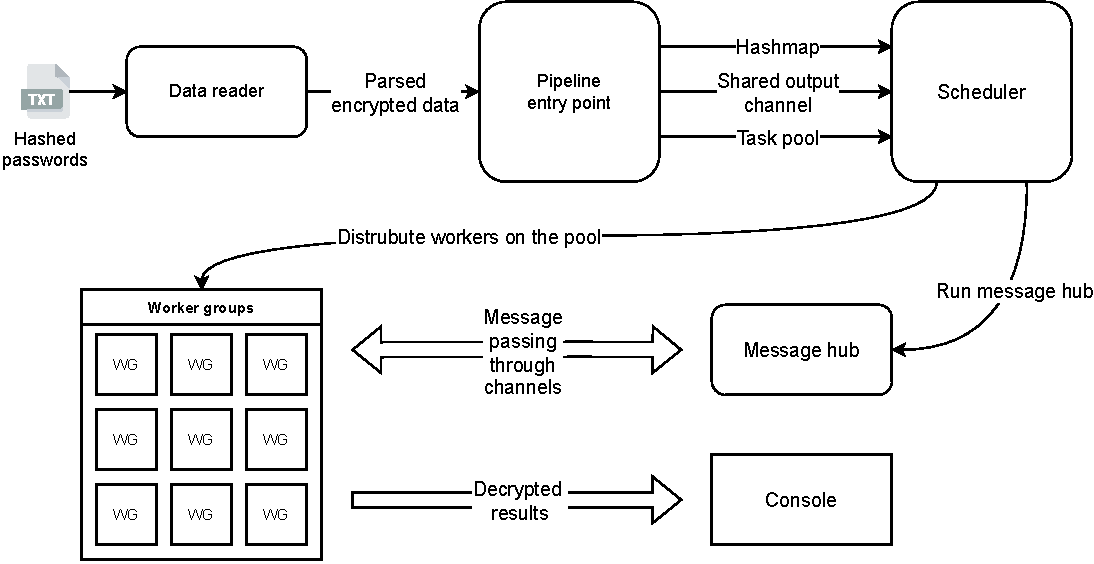
\includegraphics[width=0.8\textwidth]{resources/general_pipeline.pdf}
\end{figure}

\subsection{Worker design}

Each worker is bound to the specific disjoint subset of all lowercase letter permutations of a particular length, namely, a worker generates a unique sequence of passwords and all the workers combined generate all the passwords. To implement such a separation of computations, a worker is assigned to a particular length and the suffix of the password. Guesses are then generated starting from the lexicographically smallest permutation (e.g. \emph{aaac} if the suffix is \emph{c}) to the greatest one (e.g. \emph{zzzc}). It implies the number of workers is equal to the number of lowercase letters times the number of possible password lengths, namely $ 26 * 4 = 104 $.

\begin{figure}[h]
  \caption{Worker design}
  \vspace{0.2in}
  \centering
  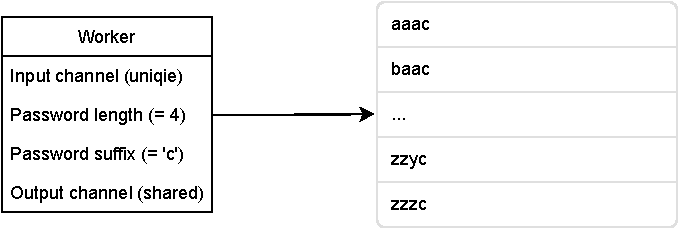
\includegraphics[width=0.6\textwidth]{resources/worker.pdf}
\end{figure}

Workers then hash generated passwords and check if their local copy of the hashmap has a key that is the digest of the generated password. If they succeed to guess a password correctly they log the decryption result to the console and send a message to the message hub which broadcasts it to the other workers. It is more efficient to generate, hash, and check passwords in place than have separate threads/tasks for these steps because excessive message passing and CPU consumption will decrease the performance noticeably.

\subsection{Scheduler implementation}

The scheduler is responsible for balancing the workload between available domains to reach the most efficient setup. It separates workers into groups based on the weight (password length) of the worker and tries to create groups that weigh similarly. Here is the output of the debug that allows observing the distribution of workers when 8 cores are used:

\begin{verbatim}
Created a task pool of 8 domains.
Workers are distributed into 7 groups:
Group1  [6; 6; 6; 6; 5; 5; 5; 5; 4; 4; 4; 3; 3; 3; 3]   (68)
Group2  [6; 6; 6; 6; 5; 5; 5; 4; 4; 4; 4; 4; 3; 3]      (65)
Group3  [6; 6; 6; 6; 5; 5; 5; 4; 4; 4; 4; 3; 3; 3; 3]   (67)
Group4  [6; 6; 6; 6; 5; 5; 5; 4; 4; 4; 4; 3; 3; 3; 3]   (67)
Group5  [6; 6; 6; 6; 5; 5; 5; 4; 4; 4; 4; 3; 3; 3; 3]   (67)
Group6  [6; 6; 6; 5; 5; 5; 5; 5; 4; 4; 4; 3; 3; 3; 3]   (67)
Group7  [6; 6; 6; 5; 5; 5; 5; 5; 4; 4; 4; 3; 3; 3; 3]   (67)
\end{verbatim}

\section{Concurrency pattern justification}

As it was mentioned above, workers are independent in terms of computations (so they do not produce collisions) which means they could be run in parallel. However, the number of workers exceeds the number of cores on most machines so a few workers are forced to share one core. To achieve parallel computations, the program makes use of OCaml domains that are mapped to physical machine cores.

It is convenient to use a task pool in order to manage domains. However, it is not a good decision to create a whole task for a worker because the number of workers is much greater than the number of domains (unless the program is run on a very powerful machine which is not the case in general). The first few workers will occupy all the available tasks and the rest will wait until they are done. But our goal is to find a small number of matching passwords as soon as possible and because we make no assumptions regarding the passwords (they are considered to be uniformly distributed) it is better to try different permutations simultaneously than spend a lot of CPU time to generate a specific sequence of passwords.

So workers should be lightweight OCaml threads that will concurrent in the scope of a core. Here comes the idea of a scheduler that finds the most optimal way to split workers into a number of even groups to run each one in a separate core. Lightweight worker threads are then bound to the domain and can run concurrently so they are not blocked by the task pool capacity. Moreover, even when the lightest workers finish (3-digit passwords probably), cores still remain balanced because the groups have similar weights. So there is no situation when one core finishes noticeably earlier than the others.

In order to check if the digest of a generated password exists in the list of data to encrypt, each worker should have an access to this list of data. Obviously, it is convenient to use a hashmap to quickly check if the digest is present or not. This data structure is not thread-safe by default so it requires to be protected by mutex if a number of concurrent workers will access it. But there is another approach that does not require process synchronization (which is very time-consuming). Every worker can maintain a local copy of the hashmap so there is no need for mutexes. Yes, it consumes more space but not too much and the performance gain outweighs the disadvantages for sure. Great, but how then workers know when to stop?

The final piece of the solution is message passing. A worker has a unique unbound channel that belongs to it and there is a hub with one unbound shared channel. If a worker wants to notify others, it may send a message to the hub channel and the hub will broadcast the message to all the workers. Channels are thread-safe so there is no data loss when two workers try to send a message simultaneously. After a worker finds a matching digest, it sends a message to the hub that is then broadcasted to the others so they can update their local copies of the hashmap or stop if all the digests were found.

\begin{figure}[h]
  \caption{Message passing}
  \vspace{0.2in}
  \centering
  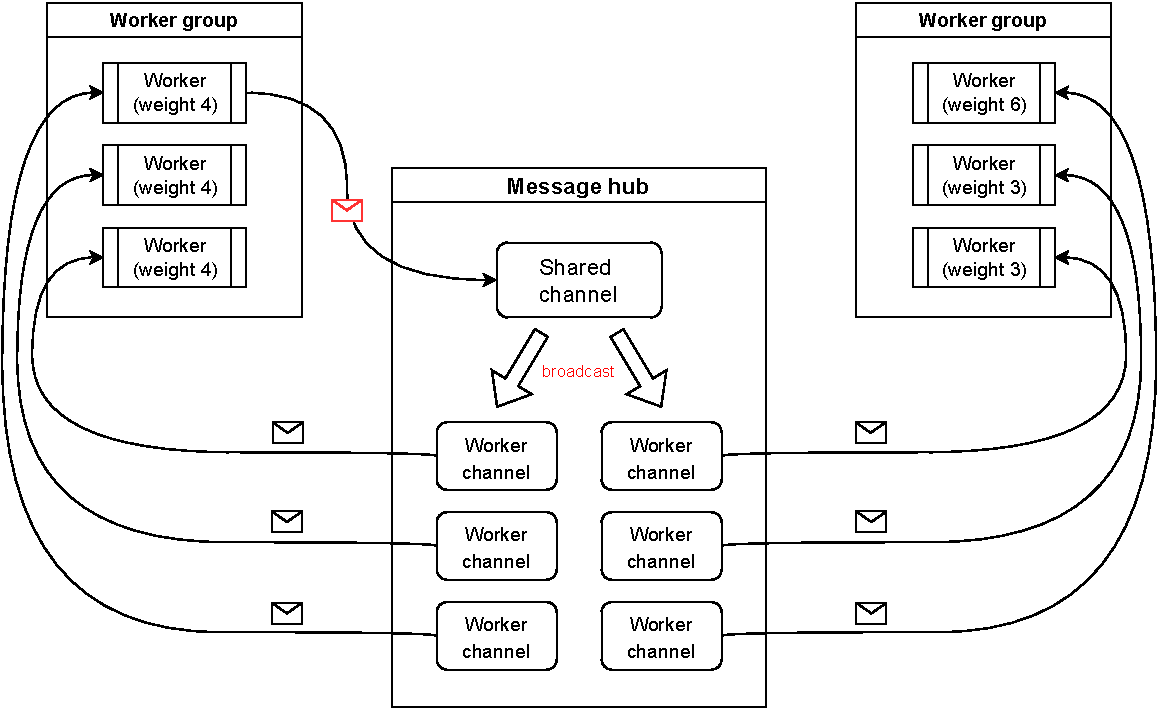
\includegraphics[width=0.8\textwidth]{resources/message_passing.pdf}
\end{figure}

\section{Benchmarking}

The default input file contains mostly 3-digit passwords that are computed very fast which makes benchmarks that use it inaccurately. However, the more balanced input file which contains passwords of different lengths and computation times shows more descriptive results.

\begin{table}[!ht]
    \centering
    \begin{tabular}{|l|l|l|l|l|}
    \hline
        Setup & Mean [s] & Min [s] & Max [s] & Relative \\ \hline
        1 core & 127.338 ± 6.511 & 115.937 & 138.516 & 8.34 ± 0.63 \\ \hline
        2 cores & 140.442 ± 13.576 & 110.433 & 154.860 & 9.20 ± 1.03 \\ \hline
        4 cores & 44.231 ± 3.321 & 40.215 & 49.686 & 2.90 ± 0.27 \\ \hline
        8 cores & 21.294 ± 0.795 & 20.286 & 22.841 & 1.40 ± 0.09 \\ \hline
        16 cores & 15.261 ± 0.854 & 14.702 & 17.551 & 1.00 \\ \hline
    \end{tabular}
\end{table}

The benchmarking was done on a machine with the following tech specs: AMD Ryzen 5800H (3.2 GHz - 4.4 GHz, 8 cores / 16 threads), and 16 GB of RAM. The command-line benchmarking tool \href{https://github.com/sharkdp/hyperfine}{\textbf{hyperfine}} is used to measure the performance of the program. Each setup is run 10 times after 5 warmup runs on the cold machine in order to reduce measurement error.

At first glance, it is obvious that parallel computations in general are more efficient. Namely, the fastest run is when all the machine threads are used. However, the speedup is not linear, so 16 domains finish not twice as fast as 8 domains. Also, it is interesting to notice that two domains are not even close to running twice as fast as a single-core setup. Moreover, it seems like this case is even slower than the non-parallel one. It might be caused by the overhead of domain creation that neglects the gained computations speedup by parallelism. When the number of domains is greater than the number of machine threads/cores, a performance decline is noticed.

Also, the optimal number of worker groups was found empirically: 
$$ worker\_groups = num\_domains - 1 $$
During benchmark runs, the $ worker\_groups = num\_domains $ setup was always slower than the previously mentioned one. It could be because the message hub is run in the same task pool as the worker groups. It seems like the message hub occupies a domain and the process takes a lot of execution time from one selected core slowing down the whole app. However, when we run one worker group less than the number of domains, the message hub takes the left domain and the workload is distributed more evenly. It is also the reason why a two-domain setup performs almost the same as a non-parallel one. Namely, only one working group is created and the message hub is run in the second domain so the program does not perform computations in parallel.

The performance gain of parallelism could be observed on the following CPU load chart. Both runs are done on the same input file but with a different number of domains. Note that even though CPU usage has increased dramatically, the execution time has not dropped by the same factor (this is also proved in the above benchmark results).

\begin{figure}[h]
  \caption{CPU load when using 4 domains and 16 domains respectively}
  \vspace{0.2in}
  \centering
  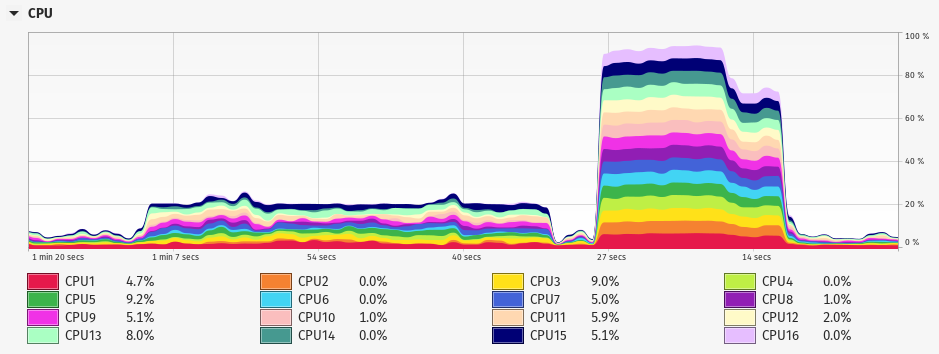
\includegraphics[width=0.9\textwidth]{resources/cpu_load.png}
\end{figure}

\section{Further improvements}

One of the most obvious points to improve is the password generation algorithm. Each worker computes a unique sequence of n-length permutations but they do this from the lexicographically smallest one to the greatest one. In other words, a password like \emph{aaaa} is generated much earlier than \emph{zzzz}. This approach is good when the passwords are distributed \emph{truly uniformly} because each password from \emph{aaaa} \emph{zzzz} then has an equal chance to appear in the input data. But in reality, this is not the case and the passwords are not evenly distributed. An algorithm to generate more popular passwords (like meaningful words) first could be used to find correct digests faster.

The program may also reuse the state between executions in some form of persistent storage. This could boost the performance in case of more difficult and long computations (longer passwords, more allowed symbols) because the program will not need to redo the same job twice.

Also, some kind of continuous data input could be implemented if the data is persistent and not erased between inputs. So the program could be a part of a more profound data pipeline that operates on live streams of data.

\end{document}